\documentclass{article}
\usepackage{iclr2027_conference}
\usepackage{graphicx}
\usepackage{booktabs}
\usepackage{amsmath}
\usepackage{amssymb}
\usepackage{amsthm}
\usepackage{multirow}
\usepackage{xcolor}
\usepackage{hyperref}
\usepackage{url}
%%%%% NEW MATH DEFINITIONS %%%%%

\usepackage{amsmath,amsfonts,bm}

% Mark sections of captions for referring to divisions of figures
\newcommand{\figleft}{{\em (Left)}}
\newcommand{\figcenter}{{\em (Center)}}
\newcommand{\figright}{{\em (Right)}}
\newcommand{\figtop}{{\em (Top)}}
\newcommand{\figbottom}{{\em (Bottom)}}
\newcommand{\captiona}{{\em (a)}}
\newcommand{\captionb}{{\em (b)}}
\newcommand{\captionc}{{\em (c)}}
\newcommand{\captiond}{{\em (d)}}

% Highlight a newly defined term
\newcommand{\newterm}[1]{{\bf #1}}


% Figure reference, lower-case.
\def\figref#1{figure~\ref{#1}}
% Figure reference, capital. For start of sentence
\def\Figref#1{Figure~\ref{#1}}
\def\twofigref#1#2{figures \ref{#1} and \ref{#2}}
\def\quadfigref#1#2#3#4{figures \ref{#1}, \ref{#2}, \ref{#3} and \ref{#4}}
% Section reference, lower-case.
\def\secref#1{section~\ref{#1}}
% Section reference, capital.
\def\Secref#1{Section~\ref{#1}}
% Reference to two sections.
\def\twosecrefs#1#2{sections \ref{#1} and \ref{#2}}
% Reference to three sections.
\def\secrefs#1#2#3{sections \ref{#1}, \ref{#2} and \ref{#3}}
% Reference to an equation, lower-case.
\def\eqref#1{equation~\ref{#1}}
% Reference to an equation, upper case
\def\Eqref#1{Equation~\ref{#1}}
% A raw reference to an equation---avoid using if possible
\def\plaineqref#1{\ref{#1}}
% Reference to a chapter, lower-case.
\def\chapref#1{chapter~\ref{#1}}
% Reference to an equation, upper case.
\def\Chapref#1{Chapter~\ref{#1}}
% Reference to a range of chapters
\def\rangechapref#1#2{chapters\ref{#1}--\ref{#2}}
% Reference to an algorithm, lower-case.
\def\algref#1{algorithm~\ref{#1}}
% Reference to an algorithm, upper case.
\def\Algref#1{Algorithm~\ref{#1}}
\def\twoalgref#1#2{algorithms \ref{#1} and \ref{#2}}
\def\Twoalgref#1#2{Algorithms \ref{#1} and \ref{#2}}
% Reference to a part, lower case
\def\partref#1{part~\ref{#1}}
% Reference to a part, upper case
\def\Partref#1{Part~\ref{#1}}
\def\twopartref#1#2{parts \ref{#1} and \ref{#2}}

\def\ceil#1{\lceil #1 \rceil}
\def\floor#1{\lfloor #1 \rfloor}
\def\1{\bm{1}}
\newcommand{\train}{\mathcal{D}}
\newcommand{\valid}{\mathcal{D_{\mathrm{valid}}}}
\newcommand{\test}{\mathcal{D_{\mathrm{test}}}}

\def\eps{{\epsilon}}


% Random variables
\def\reta{{\textnormal{$\eta$}}}
\def\ra{{\textnormal{a}}}
\def\rb{{\textnormal{b}}}
\def\rc{{\textnormal{c}}}
\def\rd{{\textnormal{d}}}
\def\re{{\textnormal{e}}}
\def\rf{{\textnormal{f}}}
\def\rg{{\textnormal{g}}}
\def\rh{{\textnormal{h}}}
\def\ri{{\textnormal{i}}}
\def\rj{{\textnormal{j}}}
\def\rk{{\textnormal{k}}}
\def\rl{{\textnormal{l}}}
% rm is already a command, just don't name any random variables m
\def\rn{{\textnormal{n}}}
\def\ro{{\textnormal{o}}}
\def\rp{{\textnormal{p}}}
\def\rq{{\textnormal{q}}}
\def\rr{{\textnormal{r}}}
\def\rs{{\textnormal{s}}}
\def\rt{{\textnormal{t}}}
\def\ru{{\textnormal{u}}}
\def\rv{{\textnormal{v}}}
\def\rw{{\textnormal{w}}}
\def\rx{{\textnormal{x}}}
\def\ry{{\textnormal{y}}}
\def\rz{{\textnormal{z}}}

% Random vectors
\def\rvepsilon{{\mathbf{\epsilon}}}
\def\rvtheta{{\mathbf{\theta}}}
\def\rva{{\mathbf{a}}}
\def\rvb{{\mathbf{b}}}
\def\rvc{{\mathbf{c}}}
\def\rvd{{\mathbf{d}}}
\def\rve{{\mathbf{e}}}
\def\rvf{{\mathbf{f}}}
\def\rvg{{\mathbf{g}}}
\def\rvh{{\mathbf{h}}}
\def\rvu{{\mathbf{i}}}
\def\rvj{{\mathbf{j}}}
\def\rvk{{\mathbf{k}}}
\def\rvl{{\mathbf{l}}}
\def\rvm{{\mathbf{m}}}
\def\rvn{{\mathbf{n}}}
\def\rvo{{\mathbf{o}}}
\def\rvp{{\mathbf{p}}}
\def\rvq{{\mathbf{q}}}
\def\rvr{{\mathbf{r}}}
\def\rvs{{\mathbf{s}}}
\def\rvt{{\mathbf{t}}}
\def\rvu{{\mathbf{u}}}
\def\rvv{{\mathbf{v}}}
\def\rvw{{\mathbf{w}}}
\def\rvx{{\mathbf{x}}}
\def\rvy{{\mathbf{y}}}
\def\rvz{{\mathbf{z}}}

% Elements of random vectors
\def\erva{{\textnormal{a}}}
\def\ervb{{\textnormal{b}}}
\def\ervc{{\textnormal{c}}}
\def\ervd{{\textnormal{d}}}
\def\erve{{\textnormal{e}}}
\def\ervf{{\textnormal{f}}}
\def\ervg{{\textnormal{g}}}
\def\ervh{{\textnormal{h}}}
\def\ervi{{\textnormal{i}}}
\def\ervj{{\textnormal{j}}}
\def\ervk{{\textnormal{k}}}
\def\ervl{{\textnormal{l}}}
\def\ervm{{\textnormal{m}}}
\def\ervn{{\textnormal{n}}}
\def\ervo{{\textnormal{o}}}
\def\ervp{{\textnormal{p}}}
\def\ervq{{\textnormal{q}}}
\def\ervr{{\textnormal{r}}}
\def\ervs{{\textnormal{s}}}
\def\ervt{{\textnormal{t}}}
\def\ervu{{\textnormal{u}}}
\def\ervv{{\textnormal{v}}}
\def\ervw{{\textnormal{w}}}
\def\ervx{{\textnormal{x}}}
\def\ervy{{\textnormal{y}}}
\def\ervz{{\textnormal{z}}}

% Random matrices
\def\rmA{{\mathbf{A}}}
\def\rmB{{\mathbf{B}}}
\def\rmC{{\mathbf{C}}}
\def\rmD{{\mathbf{D}}}
\def\rmE{{\mathbf{E}}}
\def\rmF{{\mathbf{F}}}
\def\rmG{{\mathbf{G}}}
\def\rmH{{\mathbf{H}}}
\def\rmI{{\mathbf{I}}}
\def\rmJ{{\mathbf{J}}}
\def\rmK{{\mathbf{K}}}
\def\rmL{{\mathbf{L}}}
\def\rmM{{\mathbf{M}}}
\def\rmN{{\mathbf{N}}}
\def\rmO{{\mathbf{O}}}
\def\rmP{{\mathbf{P}}}
\def\rmQ{{\mathbf{Q}}}
\def\rmR{{\mathbf{R}}}
\def\rmS{{\mathbf{S}}}
\def\rmT{{\mathbf{T}}}
\def\rmU{{\mathbf{U}}}
\def\rmV{{\mathbf{V}}}
\def\rmW{{\mathbf{W}}}
\def\rmX{{\mathbf{X}}}
\def\rmY{{\mathbf{Y}}}
\def\rmZ{{\mathbf{Z}}}

% Elements of random matrices
\def\ermA{{\textnormal{A}}}
\def\ermB{{\textnormal{B}}}
\def\ermC{{\textnormal{C}}}
\def\ermD{{\textnormal{D}}}
\def\ermE{{\textnormal{E}}}
\def\ermF{{\textnormal{F}}}
\def\ermG{{\textnormal{G}}}
\def\ermH{{\textnormal{H}}}
\def\ermI{{\textnormal{I}}}
\def\ermJ{{\textnormal{J}}}
\def\ermK{{\textnormal{K}}}
\def\ermL{{\textnormal{L}}}
\def\ermM{{\textnormal{M}}}
\def\ermN{{\textnormal{N}}}
\def\ermO{{\textnormal{O}}}
\def\ermP{{\textnormal{P}}}
\def\ermQ{{\textnormal{Q}}}
\def\ermR{{\textnormal{R}}}
\def\ermS{{\textnormal{S}}}
\def\ermT{{\textnormal{T}}}
\def\ermU{{\textnormal{U}}}
\def\ermV{{\textnormal{V}}}
\def\ermW{{\textnormal{W}}}
\def\ermX{{\textnormal{X}}}
\def\ermY{{\textnormal{Y}}}
\def\ermZ{{\textnormal{Z}}}

% Vectors
\def\vzero{{\bm{0}}}
\def\vone{{\bm{1}}}
\def\vmu{{\bm{\mu}}}
\def\vtheta{{\bm{\theta}}}
\def\va{{\bm{a}}}
\def\vb{{\bm{b}}}
\def\vc{{\bm{c}}}
\def\vd{{\bm{d}}}
\def\ve{{\bm{e}}}
\def\vf{{\bm{f}}}
\def\vg{{\bm{g}}}
\def\vh{{\bm{h}}}
\def\vi{{\bm{i}}}
\def\vj{{\bm{j}}}
\def\vk{{\bm{k}}}
\def\vl{{\bm{l}}}
\def\vm{{\bm{m}}}
\def\vn{{\bm{n}}}
\def\vo{{\bm{o}}}
\def\vp{{\bm{p}}}
\def\vq{{\bm{q}}}
\def\vr{{\bm{r}}}
\def\vs{{\bm{s}}}
\def\vt{{\bm{t}}}
\def\vu{{\bm{u}}}
\def\vv{{\bm{v}}}
\def\vw{{\bm{w}}}
\def\vx{{\bm{x}}}
\def\vy{{\bm{y}}}
\def\vz{{\bm{z}}}

% Elements of vectors
\def\evalpha{{\alpha}}
\def\evbeta{{\beta}}
\def\evepsilon{{\epsilon}}
\def\evlambda{{\lambda}}
\def\evomega{{\omega}}
\def\evmu{{\mu}}
\def\evpsi{{\psi}}
\def\evsigma{{\sigma}}
\def\evtheta{{\theta}}
\def\eva{{a}}
\def\evb{{b}}
\def\evc{{c}}
\def\evd{{d}}
\def\eve{{e}}
\def\evf{{f}}
\def\evg{{g}}
\def\evh{{h}}
\def\evi{{i}}
\def\evj{{j}}
\def\evk{{k}}
\def\evl{{l}}
\def\evm{{m}}
\def\evn{{n}}
\def\evo{{o}}
\def\evp{{p}}
\def\evq{{q}}
\def\evr{{r}}
\def\evs{{s}}
\def\evt{{t}}
\def\evu{{u}}
\def\evv{{v}}
\def\evw{{w}}
\def\evx{{x}}
\def\evy{{y}}
\def\evz{{z}}

% Matrix
\def\mA{{\bm{A}}}
\def\mB{{\bm{B}}}
\def\mC{{\bm{C}}}
\def\mD{{\bm{D}}}
\def\mE{{\bm{E}}}
\def\mF{{\bm{F}}}
\def\mG{{\bm{G}}}
\def\mH{{\bm{H}}}
\def\mI{{\bm{I}}}
\def\mJ{{\bm{J}}}
\def\mK{{\bm{K}}}
\def\mL{{\bm{L}}}
\def\mM{{\bm{M}}}
\def\mN{{\bm{N}}}
\def\mO{{\bm{O}}}
\def\mP{{\bm{P}}}
\def\mQ{{\bm{Q}}}
\def\mR{{\bm{R}}}
\def\mS{{\bm{S}}}
\def\mT{{\bm{T}}}
\def\mU{{\bm{U}}}
\def\mV{{\bm{V}}}
\def\mW{{\bm{W}}}
\def\mX{{\bm{X}}}
\def\mY{{\bm{Y}}}
\def\mZ{{\bm{Z}}}
\def\mBeta{{\bm{\beta}}}
\def\mPhi{{\bm{\Phi}}}
\def\mLambda{{\bm{\Lambda}}}
\def\mSigma{{\bm{\Sigma}}}

% Tensor
\DeclareMathAlphabet{\mathsfit}{\encodingdefault}{\sfdefault}{m}{sl}
\SetMathAlphabet{\mathsfit}{bold}{\encodingdefault}{\sfdefault}{bx}{n}
\newcommand{\tens}[1]{\bm{\mathsfit{#1}}}
\def\tA{{\tens{A}}}
\def\tB{{\tens{B}}}
\def\tC{{\tens{C}}}
\def\tD{{\tens{D}}}
\def\tE{{\tens{E}}}
\def\tF{{\tens{F}}}
\def\tG{{\tens{G}}}
\def\tH{{\tens{H}}}
\def\tI{{\tens{I}}}
\def\tJ{{\tens{J}}}
\def\tK{{\tens{K}}}
\def\tL{{\tens{L}}}
\def\tM{{\tens{M}}}
\def\tN{{\tens{N}}}
\def\tO{{\tens{O}}}
\def\tP{{\tens{P}}}
\def\tQ{{\tens{Q}}}
\def\tR{{\tens{R}}}
\def\tS{{\tens{S}}}
\def\tT{{\tens{T}}}
\def\tU{{\tens{U}}}
\def\tV{{\tens{V}}}
\def\tW{{\tens{W}}}
\def\tX{{\tens{X}}}
\def\tY{{\tens{Y}}}
\def\tZ{{\tens{Z}}}


% Graph
\def\gA{{\mathcal{A}}}
\def\gB{{\mathcal{B}}}
\def\gC{{\mathcal{C}}}
\def\gD{{\mathcal{D}}}
\def\gE{{\mathcal{E}}}
\def\gF{{\mathcal{F}}}
\def\gG{{\mathcal{G}}}
\def\gH{{\mathcal{H}}}
\def\gI{{\mathcal{I}}}
\def\gJ{{\mathcal{J}}}
\def\gK{{\mathcal{K}}}
\def\gL{{\mathcal{L}}}
\def\gM{{\mathcal{M}}}
\def\gN{{\mathcal{N}}}
\def\gO{{\mathcal{O}}}
\def\gP{{\mathcal{P}}}
\def\gQ{{\mathcal{Q}}}
\def\gR{{\mathcal{R}}}
\def\gS{{\mathcal{S}}}
\def\gT{{\mathcal{T}}}
\def\gU{{\mathcal{U}}}
\def\gV{{\mathcal{V}}}
\def\gW{{\mathcal{W}}}
\def\gX{{\mathcal{X}}}
\def\gY{{\mathcal{Y}}}
\def\gZ{{\mathcal{Z}}}

% Sets
\def\sA{{\mathbb{A}}}
\def\sB{{\mathbb{B}}}
\def\sC{{\mathbb{C}}}
\def\sD{{\mathbb{D}}}
% Don't use a set called E, because this would be the same as our symbol
% for expectation.
\def\sF{{\mathbb{F}}}
\def\sG{{\mathbb{G}}}
\def\sH{{\mathbb{H}}}
\def\sI{{\mathbb{I}}}
\def\sJ{{\mathbb{J}}}
\def\sK{{\mathbb{K}}}
\def\sL{{\mathbb{L}}}
\def\sM{{\mathbb{M}}}
\def\sN{{\mathbb{N}}}
\def\sO{{\mathbb{O}}}
\def\sP{{\mathbb{P}}}
\def\sQ{{\mathbb{Q}}}
\def\sR{{\mathbb{R}}}
\def\sS{{\mathbb{S}}}
\def\sT{{\mathbb{T}}}
\def\sU{{\mathbb{U}}}
\def\sV{{\mathbb{V}}}
\def\sW{{\mathbb{W}}}
\def\sX{{\mathbb{X}}}
\def\sY{{\mathbb{Y}}}
\def\sZ{{\mathbb{Z}}}

% Entries of a matrix
\def\emLambda{{\Lambda}}
\def\emA{{A}}
\def\emB{{B}}
\def\emC{{C}}
\def\emD{{D}}
\def\emE{{E}}
\def\emF{{F}}
\def\emG{{G}}
\def\emH{{H}}
\def\emI{{I}}
\def\emJ{{J}}
\def\emK{{K}}
\def\emL{{L}}
\def\emM{{M}}
\def\emN{{N}}
\def\emO{{O}}
\def\emP{{P}}
\def\emQ{{Q}}
\def\emR{{R}}
\def\emS{{S}}
\def\emT{{T}}
\def\emU{{U}}
\def\emV{{V}}
\def\emW{{W}}
\def\emX{{X}}
\def\emY{{Y}}
\def\emZ{{Z}}
\def\emSigma{{\Sigma}}

% entries of a tensor
% Same font as tensor, without \bm wrapper
\newcommand{\etens}[1]{\mathsfit{#1}}
\def\etLambda{{\etens{\Lambda}}}
\def\etA{{\etens{A}}}
\def\etB{{\etens{B}}}
\def\etC{{\etens{C}}}
\def\etD{{\etens{D}}}
\def\etE{{\etens{E}}}
\def\etF{{\etens{F}}}
\def\etG{{\etens{G}}}
\def\etH{{\etens{H}}}
\def\etI{{\etens{I}}}
\def\etJ{{\etens{J}}}
\def\etK{{\etens{K}}}
\def\etL{{\etens{L}}}
\def\etM{{\etens{M}}}
\def\etN{{\etens{N}}}
\def\etO{{\etens{O}}}
\def\etP{{\etens{P}}}
\def\etQ{{\etens{Q}}}
\def\etR{{\etens{R}}}
\def\etS{{\etens{S}}}
\def\etT{{\etens{T}}}
\def\etU{{\etens{U}}}
\def\etV{{\etens{V}}}
\def\etW{{\etens{W}}}
\def\etX{{\etens{X}}}
\def\etY{{\etens{Y}}}
\def\etZ{{\etens{Z}}}

% The true underlying data generating distribution
\newcommand{\pdata}{p_{\rm{data}}}
% The empirical distribution defined by the training set
\newcommand{\ptrain}{\hat{p}_{\rm{data}}}
\newcommand{\Ptrain}{\hat{P}_{\rm{data}}}
% The model distribution
\newcommand{\pmodel}{p_{\rm{model}}}
\newcommand{\Pmodel}{P_{\rm{model}}}
\newcommand{\ptildemodel}{\tilde{p}_{\rm{model}}}
% Stochastic autoencoder distributions
\newcommand{\pencode}{p_{\rm{encoder}}}
\newcommand{\pdecode}{p_{\rm{decoder}}}
\newcommand{\precons}{p_{\rm{reconstruct}}}

\newcommand{\laplace}{\mathrm{Laplace}} % Laplace distribution

\newcommand{\E}{\mathbb{E}}
\newcommand{\Ls}{\mathcal{L}}
\newcommand{\R}{\mathbb{R}}
\newcommand{\emp}{\tilde{p}}
\newcommand{\lr}{\alpha}
\newcommand{\reg}{\lambda}
\newcommand{\rect}{\mathrm{rectifier}}
\newcommand{\softmax}{\mathrm{softmax}}
\newcommand{\sigmoid}{\sigma}
\newcommand{\softplus}{\zeta}
\newcommand{\KL}{D_{\mathrm{KL}}}
\newcommand{\Var}{\mathrm{Var}}
\newcommand{\standarderror}{\mathrm{SE}}
\newcommand{\Cov}{\mathrm{Cov}}
% Wolfram Mathworld says $L^2$ is for function spaces and $\ell^2$ is for vectors
% But then they seem to use $L^2$ for vectors throughout the site, and so does
% wikipedia.
\newcommand{\normlzero}{L^0}
\newcommand{\normlone}{L^1}
\newcommand{\normltwo}{L^2}
\newcommand{\normlp}{L^p}
\newcommand{\normmax}{L^\infty}

\newcommand{\parents}{Pa} % See usage in notation.tex. Chosen to match Daphne's book.

\DeclareMathOperator*{\argmax}{arg\,max}
\DeclareMathOperator*{\argmin}{arg\,min}

\DeclareMathOperator{\sign}{sign}
\DeclareMathOperator{\Tr}{Tr}
\let\ab\allowbreak


\newtheorem{proposition}{Proposition}
\newtheorem{remark}{Remark}
\newtheorem{definition}{Definition}

\newcommand{\TBD}[1]{\textcolor{red}{\textbf{[TBD: #1]}}}
\newcommand{\gap}{g_{\mathrm{oracle}}}
\newcommand{\rfc}{RegionFocal}

\title{Not All Smoothness Is Fixable:\\Diagnosing and Conditionally Repairing Over-Smoothing\\in Time Series Forecasting}

\author{Anonymous Authors}

\begin{document}
\maketitle

\begin{abstract}
Point forecasts trained with mean squared error are systematically smoother than the series they predict, and a long line of work treats this over-smoothing as a defect to be repaired. We ask a prior question: is the observed smoothness always fixable? We decompose the future into a predictable conditional mean and an irreducible noise term, and show that the Bayes-optimal forecast must already look smoother than any realized series. Over-smoothing therefore has two components: rational shrinkage, which is the optimal response to uncertainty, and unexploited structure, which is repairable. We operationalize the distinction with the \emph{oracle gap}, a training-free diagnostic that simulates the signature an oracle would exhibit on a given dataset and compares it with the signature of a trained model. Across 14 dataset-model cells and a 665-cell audit of 13 time-series foundation models on 50 benchmark variants, the oracle gap predicts when anti-smoothing interventions help, with no contradictory cell. We then introduce \rfc, a region-weighted loss that up-weights points where the prediction under-shoots the realized amplitude. Guided by the diagnostic, \rfc~reduces MSE by 2.3\% on Electricity across three seeds and four horizons, and degrades gracefully to the MSE baseline exactly where the gap is non-positive. For regimes where smoothing is rational, we show that a light-weight descriptor head that predicts structural properties of the future window cannot repair point accuracy, but provides a reliable forward-looking signal for selective prediction: abstaining on the 20\% highest-risk windows reduces the remaining MSE by up to 5.3\%. Our results replace a blanket intuition about over-smoothing with a measurable and predictable condition for when it is worth fixing.
\end{abstract}

\section{Introduction}

Deep forecasters trained with mean squared error produce predictions that are visibly smoother than the series they imitate: a well-tuned PatchTST on ETTh1 predicts with an amplitude ratio of 0.84 relative to the realized series, and half of its point predictions fall strictly between a level reference and the realized value. This signature is widely treated as a defect: frequency-domain losses attribute it to label autocorrelation \citep{fredf}, auxiliary classification heads to the failure of squared losses on high-entropy features \citep{hcan}, and shape-aware objectives penalize it directly \citep{dilate}---all premised on the smoothness being pathological and repair improving accuracy.

This premise needs qualification. A squared-loss-optimal forecast is the conditional mean of the future given the context, which is necessarily smoother than any realization, because realizations contain unpredictable noise that no point forecast should imitate: the over-smoothing signature is a property of the optimal predictor itself, not only of imperfect models. Whether a trained model is \emph{too} smooth depends on how its signature compares with the signature an oracle would leave on the same data. This reframing decomposes over-smoothing into \emph{rational shrinkage}, which an optimal predictor must keep, and \emph{unexploited structure}, which can in principle be repaired.

We make the decomposition measurable. Our diagnostic, the \emph{oracle gap}, bootstraps a trained model's residuals to synthesize alternative realizations of the future and compares the amplitude signature the model's predictions would exhibit as an oracle against them with the signature observed against the true data. The gap needs no training and runs in seconds per cell: positive indicates residuals with structure the model failed to extract, non-positive indicates rational shrinkage.

The diagnostic is predictive, not just descriptive: across fifteen dataset-backbone cells, the sign of the gap predicts the sign of the intervention's effect in all but one cell (14/15, $p < 5 \times 10^{-4}$ under a sign-symmetric null); the exception is diagnosable in advance from the anchor geometry. A separate 665-cell audit of thirteen foundation models and a trained PatchTST on fifty GIFT-Eval variants \citep{gifteval} corroborates from the accuracy side, and settles several folk questions: ETT is saturated, transit and energy series retain exploitable structure across all thirteen models, scale is irrelevant from 8M to 311M parameters, and accuracy rank anti-correlates with leftover structure.

Guided by the diagnostic, we introduce \rfc, a region-weighted loss that increases the penalty where the prediction under-shoots the realized deviation from a level reference while leaving the zero-loss set of MSE untouched; a Gaussian analysis bounds the induced fixed-point shift at roughly $0.4\alpha\sigma$, so the loss acts as a calibrated counter-bias rather than a new objective. On Electricity, \rfc~reduces MSE by 2.3\% across three seeds and horizons from 96 to 720 steps; on non-positive-gap datasets the diagnostic withholds the repair, avoiding the harm it would otherwise cause.

Where shrinkage is rational, a model can still be made more useful by knowing when it is likely to fail. A light-weight descriptor head predicts structural properties of the future window, with labels computed for free from training data. Such heads cannot repair point accuracy at the scales we study, echoing scale-dependent findings for multi-token prediction \citep{gloeckle2024mtp,fsf}, but the predicted change-point probability is a reliable forward-looking risk signal: abstaining on the 20\% highest-risk windows reduces the remaining MSE by up to 5.3\% on task models and 9.6\% on a fine-tuned foundation model, outperforming oracle change-point rankings and static baselines. Predicting future structure is more useful for deciding when to trust a forecast than for improving it.

\textbf{Contributions.}
\begin{itemize}\setlength\itemsep{1pt}
    \item A two-component theory of over-smoothing---rational shrinkage versus unexploited structure---with a conditional improvement interval $(0, 2b)$ and a Jensen-gap argument for supervising structure through auxiliary heads.
    \item The oracle gap, a training-free diagnostic of repairable structure: its sign predicts intervention outcomes in 14 of 15 cells (the exception has an identified geometric cause), corroborated by a 665-cell audit.
    \item \rfc, a region-weighted loss that repairs over-smoothing where the diagnostic is positive and is withheld where it would harm, with a bounded fixed-point shift.
    \item An audit of forecasting benchmarks through repairable structure: saturation evidence for ETT, positive cells in transit and energy series, and flat scaling across model size.
    \item Evidence that predicted structural descriptors are more valuable at decision time than at training time, including a selective-prediction gain of 5.3\% exceeding oracle change-point ranking.
\end{itemize}

\section{Related Work}

\paragraph{Over-smoothing and loss design in forecasting.}
Squared-error training shrinks forecasts toward conditional means, and several works repair the resulting smoothness. FreDF trains in the frequency domain to decorrelate label-autocorrelation bias \citep{fredf}, with follow-ups on learnable or orthogonalized transform domains \citep{transdf,olinear,fredn}. HCAN attaches hierarchical classification over binned amplitudes to preserve high-entropy features \citep{hcan}, and DILATE penalizes shape and temporal distortion directly \citep{dilate}. Asymmetric losses \citep{newey1987expectile,zellner1986linex} penalize over- and under-prediction differently, and focal weighting schemes up-weight hard examples in imbalanced prediction problems \citep{focal_loss,lds_fds}. These methods intervene unconditionally; we instead characterize when repair is possible at all. \rf~is closest to this reweighting family, but its weights are conditioned on the prediction's position relative to a level reference and the realization, targeting under-dispersion rather than sign asymmetry or example difficulty. A complementary theoretical result bounds what any deterministic forecast can achieve: under nonzero conditional uncertainty, no predictor can simultaneously minimize MSE and match the marginal distribution of realized futures, and the attainable accuracy--realism pairs form a Pareto frontier \citep{green2026expectations}. That work maps the frontier; we ask which positions on it are reachable by training-time intervention, and measure the remaining headroom per dataset--model pair.

\paragraph{Forward-looking supervision.}
Multi-token prediction trains language models to predict several future tokens from one hidden state, with scale-dependent gains \citep{gloeckle2024mtp,mutor}, and future-summary prediction replaces token values with compact summaries of the long-term future \citep{fsf}. Our descriptor head shares the motivation that future supervision should be denser than next-step values, but differs in target (structural statistics of continuous series), objective geometry (squared-loss forecasting), and use (an inference-time decision signal). Moirai 2.0 adopts patch-level multi-token prediction for decoding efficiency \citep{moirai2}, without a decision-time reading.

\paragraph{Uncertainty, abstention, and conformal prediction.}
Adaptive conformal inference maintains coverage under distribution shift \citep{gibbs2021aci,gibbs2024dtaci}, and CPTC anticipates change points with an exogenous state-transition model \citep{cptc}. Reject-option forecasting is comparatively underexplored \citep{boundedabstention,rejectoptiontsf}. Our selective-prediction signal is endogenous and free: it is read from a descriptor head trained on labels computed from the future window itself.
\paragraph{Benchmark auditing.}
GIFT-Eval ranks forecasters across many datasets \citep{gifteval}; our audit is orthogonal, measuring how much repairable structure each dataset--model pair leaves behind and where accuracy interventions can still help.

\section{The Two Components of Over-Smoothing}
\label{sec:theory}

\subsection{Setup}

Let $x \in \mathbb{R}^{L_0 \times C}$ be a context window and $y \in \mathbb{R}^{H \times C}$ the future window. A forecaster $\hat{y} = f(x)$ is trained with squared error. Decompose the future as
\begin{equation}
    y = \mu(x) + \varepsilon, \qquad \mu(x) = \mathbb{E}[y \mid x],
    \label{eq:decomp}
\end{equation}
where $\varepsilon$ is unpredictable from the context, with $\mathbb{E}[\varepsilon \mid x] = 0$ and conditional covariance $\Sigma(x)$. The population-optimal forecast under squared error is $\hat{y}^\star = \mu(x)$.

\subsection{The optimal predictor already looks over-smoothed}

Fix a level reference $m$ from the context, for example the per-channel context mean. A prediction point \emph{under-shoots} when $\hat{y}$ lies strictly between $m$ and $y$; dispersion is measured by the amplitude ratio $\mathrm{std}(\hat{y}) / \mathrm{std}(y)$.

\begin{proposition}[Oracle under-shooting]
\label{prop:oracle}
Under \eqref{eq:decomp}, the Bayes-optimal forecast satisfies
\begin{equation}
    \mathbb{E}\|\hat{y}^\star - m\|^2 = \mathbb{E}\|y - m\|^2 - \mathrm{tr}\,\Sigma(x) \; < \; \mathbb{E}\|y - m\|^2
\end{equation}
whenever $\mathrm{tr}\,\Sigma(x) > 0$. Hence $\mathrm{std}(\hat{y}^\star) / \mathrm{std}(y) \le \sqrt{1 - \bar{\sigma}^2 / \mathrm{Var}(y)}$, where $\bar{\sigma}^2$ is the mean conditional noise variance. When unpredictable noise is present, the optimal forecast has strictly smaller amplitude than the realized series, and its under-shoot rate is a property of the oracle, not a symptom of model failure.
\end{proposition}

The practical content is a warning: comparing a trained forecast with realized series will always find under-shooting, even for the optimal model. Over-smoothing claims require a reference for how smooth an oracle \emph{would} look on the same data; Section~\ref{sec:diagnostic} constructs one by simulation.

\subsection{Rational shrinkage versus unexploited structure}

Write the model's conditional bias as $b(x) = \mu(x) - \mathbb{E}[\hat{y} \mid x]$. The model exhibits \emph{rational shrinkage} where $b(x) \approx 0$ yet its amplitude ratio is below one, and \emph{unexploited structure} where $b(x)$ correlates with predictable structure in $y$, such as regime changes visible in the context.

\begin{proposition}[Conditional improvement interval]
\label{prop:interval}
Let $\hat{y}_\delta = \hat{y} + \delta(x)$ add a deterministic counter-bias of magnitude $\delta$ opposite to the shrinkage bias $b(x)$. Then
\begin{equation}
    \Delta \mathcal{L} = |\delta|^2 - 2\langle \delta, b \rangle
    \label{eq:counterbias}
\end{equation}
is strictly negative whenever $0 < |\delta| < 2|b| \cos\theta$, where $\theta$ is the angle between correction and bias. The optimal correction $\delta^\star = b$ removes the shrinkage bias exactly.
\end{proposition}

Equation~\eqref{eq:counterbias} separates three regimes. When $b$ is large and aligned with the correction, a positive interval of beneficial strengths exists. When $b \approx 0$, any correction costs $|\delta|^2$. When the correction is misaligned with the bias, for example when a channel-mixing architecture rotates the correction in function space, only the cost remains. All three regimes appear in our experiments, and the oracle gap identifies the first in advance.

\subsection{Why structure belongs in auxiliary heads, not on the output}

Requiring the forecast to match structural descriptors of the realized future, such as volatility or spectral entropy, is tempting. For linear descriptors $D$ such as trend slope, $D(\mathbb{E}[y \mid x]) = \mathbb{E}[D(y) \mid x]$, so matching is compatible with the conditional mean. For nonlinear descriptors, Jensen's inequality gives $D(\mathbb{E}[y \mid x]) \neq \mathbb{E}[D(y) \mid x]$ in general, and matching realized values on the output pulls the forecast away from the conditional mean exactly where the descriptor is informative. Supervising structure through an auxiliary head keeps the main output's optimum intact while shaping the shared representation.

\begin{remark}[No free reweighting]
\label{rem:impossible}
Any per-point weight $w(\hat{y}, y)$ correlated with the residual $y - \mu(x)$ moves the population minimizer away from $\mu(x)$, while a weight uncorrelated with the residual cannot target under-dispersion. The choice is between a controlled bias and none; we make the controlled bias explicit and bounded in Section~\ref{sec:regionfocal}.
\end{remark}

\subsection{A Gaussian fixed-point analysis}

Let $y \mid x \sim \mathcal{N}(\mu, \sigma^2)$, anchor $m < \mu$, and consider $\mathbb{E}[(1 + \alpha\,\mathbf{1}[y > c])(c - y)^2]$ over a constant prediction $c$. The fixed point satisfies
\begin{equation}
    c^\star = \mu + \frac{\alpha\,\sigma\,\varphi(0)}{1 + \alpha / 2} + O(\alpha^2) \;\approx\; \mu + \frac{0.4\,\alpha\,\sigma}{1 + \alpha/2},
    \label{eq:fixedpoint}
\end{equation}
so the counter-bias moves the optimum away from the anchor by an amount proportional to $\alpha\sigma$ with bounded slope. When the anchor coincides with $\mu$, the objective develops two symmetric minima flanking it, so the anchor also controls the correction's symmetry. Derivations are in Appendix~\ref{app:proofs}.

\section{The Oracle Gap Diagnostic}
\label{sec:diagnostic}

\subsection{Definition}

Proposition~\ref{prop:oracle} implies that a trained model's amplitude signature is meaningful only relative to the signature an oracle would produce on the same data. We cannot observe the oracle, but we can simulate how the model's own predictions would score as one. Let $\{\hat{y}_i, y_i\}_{i=1}^{N}$ be test-window forecasts and realizations, and let $r_i = y_i - \hat{y}_i$ be the residual windows. If the model captured all predictable structure, residuals would be exchangeable across windows, and $\hat{y}_i$ would act as the conditional mean of a fresh realization $\tilde{y}_i = \hat{y}_i + r_{\pi(i)}$ for a random permutation $\pi$. We define
\begin{equation}
    \gap \;=\; \mathbb{E}_{\pi}\!\left[\frac{\mathrm{std}(\hat{y})}{\mathrm{std}(\tilde{y})}\right] \;-\; \frac{\mathrm{std}(\hat{y})}{\mathrm{std}(y)},
    \label{eq:gap}
\end{equation}
where standard deviations are computed per window and channel around the context-mean anchor and then pooled. The first term is the amplitude ratio the model would exhibit as an oracle; the second is the observed ratio. A positive gap means the model under-shoots more against the true future than against realizations consistent with its own residuals, so the residuals still contain window-specific, non-exchangeable structure. A gap near zero means the residuals behave like noise and the shrinkage is rational.

\subsection{Protocol and robustness}

We compute \eqref{eq:gap} with twenty bootstrap repetitions; confidence intervals are below $\pm 0.005$ throughout. Statistics are computed after per-window, per-channel standardization so large-scale series do not dominate, and evaluation uses a fixed tail protocol (the last $96{+}96$ steps of each series) because the gap is sensitive to the window set. Appendix~\ref{app:diagnostic} reports anchor and window-set sensitivity. The diagnostic is training-free and costs seconds per cell.

The simulation uses the model's own predictions as a proxy for the conditional mean, which makes the diagnostic one-sidedly conservative: if the model is under-dispersed relative to the true conditional mean, the simulated oracle inherits the same under-dispersion, so the true gap can only be larger than the measured one. The estimate is thus a lower bound on repairable structure; a residual that is structured but wrong would evade detection, and the audit's 680 uncontradicted cells bound that risk empirically.

\subsection{Reading the gap}

Three signatures recur. A positive gap, as on Electricity ($+0.030$) and Traffic ($+0.027$), marks residuals with leftover structure and predicts that anti-smoothing interventions help. A gap near zero, as on all four ETT series ($-0.02$ to $-0.04$) and SWaT ($+0.006$), marks rational shrinkage and predicts neutral or harmful interventions. A strongly negative gap, as on Jena weather ($-0.058$), indicates a model already over-dispersed relative to its residual oracle, where amplitude pressure accelerates the harm. Section~\ref{sec:law} shows these predictions hold in every cell we tested.

\begin{remark}[Consistency]
Under window-level exchangeability of residuals in the absence of leftover structure, the permutation estimate concentrates on the exchangeable signature as the number of windows grows, so the gap is a consistent test of residual non-exchangeability under that null. We use it as a signed magnitude rather than only a test, and the law in Section~\ref{sec:law} is the empirical warrant for that stronger use.
\end{remark}

Probing hidden states measures what a model \emph{contains}; the oracle gap measures what its residuals \emph{still lack} (Appendix~\ref{app:negative}).

\section{The Repair Decision: Diagnosing When Anti-Smoothing Helps}
\label{sec:law}

The oracle gap is one branch of a repair decision; Section~\ref{sec:regionfocal} completes the tree with the level-lag regime. Cells are routed by the residual's dominant bias type, measured by the signed residual effect size $|\mathbb{E}[r]|/\mathrm{std}(r)$ over the test windows: dispersion-dominated cells are gated by the oracle gap here, while lag-dominated cells are analyzed in Section~\ref{sec:regionfocal}. The two regimes separate bimodally on every cell we tested---at most $0.052$ on the dispersion cells of Table~\ref{tab:law} and at least $0.110$ on the lag cells of Section~\ref{sec:regionfocal}---so no conclusion depends on the routing threshold. We evaluate the pairing of the oracle gap with \rfc~(Section~\ref{sec:regionfocal}) on sixteen dispersion-regime dataset-backbone cells, eleven across nine datasets in Table~\ref{tab:law} and five across backbones in Appendix~\ref{app:matrix}. The sign of the gap predicts the direction of the intervention's effect on fifteen of the sixteen cells, counting changes within $\pm 0.5\%$ as neutral; the single exception is analyzed below. The two largest gaps give the largest improvements and all non-positive gaps give neutral or negative effects; the magnitude relation is monotone but coarse, and we treat the sign, not the magnitude, as the diagnostic's decision variable. Under a sign-symmetric null the probability of fifteen or more sign-consistent cells out of sixteen is below $3 \times 10^{-4}$, so the gate is a statistical regularity, not a coincidence.

\begin{table}[t]
  \footnotesize
  \caption{The oracle gap predicts the effect of dispersion-targeting repair (\rfc). Negative relative MSE change is better. Multi-seed cells report the mean over seeds 2021--2023, single-seed cells use seed 2021; Traffic cells use $\alpha{=}0.5$ (the development-selected value, Table~\ref{tab:main}) and all others $\alpha{=}1$. $\dagger$: descriptor-head variant.}
  \label{tab:law}
  \centering
  \begin{tabular}{llccc}
    \toprule
    Dataset & Backbone & Oracle gap & $\Delta$MSE (\%) & Prediction \\
    \midrule
    Electricity & PatchTST & $+0.030$ & $-2.3$ & \checkmark \\
    Traffic & PatchTST & $+0.027$ & $-1.0$ & \checkmark \\
    Traffic & iTransformer & $-0.023$ & $+4.4$ & \checkmark \\
    Traffic & FreTS & $+0.013$ & $+0.9$ & $\times$ \\
    solar/H & PatchTST & $+0.017$ & $-2.5$ & \checkmark \\
    SWaT & PatchTST & $+0.006$ & $+0.1$ & \checkmark \\
    bizitobs\_app. & PatchTST & $+0.009$ & $-1.7$ & \checkmark \\
    SZ\_TAXI & PatchTST & $-0.010$ & $+0.4$ & \checkmark \\
    ETTh1 & PatchTST & $-0.022$ & $+2.6$ & \checkmark \\
    ETTm1 & PatchTST & $-0.023$ & $-0.2$ & \checkmark \\
    Weather & PatchTST & $-0.058$ & $+2.5^{\dagger}$ & \checkmark \\
    \bottomrule
  \end{tabular}
\end{table}

The same law holds across five backbone families on Electricity (Appendix~\ref{app:matrix}, Table~\ref{tab:backbone}): the per-backbone gap, not the architecture family, orders the outcomes. The single sign-rule exception is FreTS on Traffic (gap $+0.013$, effect $+0.9 \pm 0.1\%$ across three seeds). It is diagnosable in advance: its under-shoot region does not dominate (rate $0.47$ versus $\ge 0.55$ on every improving dispersion cell), so up-weighting it barely shifts the gradient balance, and its signed bias concentrates in a minority of windows (top decile $59\%$, versus $11$--$18\%$ on the m4\_weekly cells); MAE fails there as well ($+4.7\%$). Both statistics are computable from a baseline run before any repair is trained (Appendix~\ref{app:negative}).

\subsection{A 665-cell audit of foundation models}
\label{sec:tsfmmap}

We extend the audit to thirteen zero-shot time-series foundation models, Chronos-Bolt at four scales (8M, 21M, 48M, 205M), Chronos-2, Sundial, Moirai-1.1 at two scales, Moirai-2.0, TimeMoE at two scales, Timer, and TiRex, on fifty dataset variants from GIFT-Eval \citep{gifteval} under the tail protocol. Figure~\ref{fig:map} summarizes the map.

\begin{figure}[t]
  \centering
  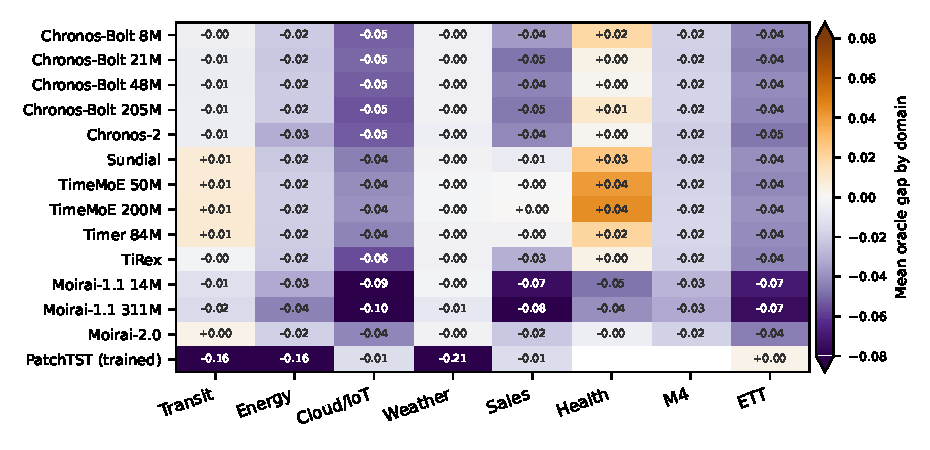
\includegraphics[width=\linewidth,height=3.4cm,keepaspectratio]{figures/fig_map_domain.pdf}
  \caption{Oracle gap aggregated by domain and model (means over the dataset variants within each domain). Positive gaps concentrate in transit and health series and are consistent across models; ETT variants are negative everywhere; the gap is flat across model scale. The two most positive single variants are SZ\_TAXI/15T ($+0.072$) and bizitobs\_application ($+0.067$); the full fifty-variant heatmap is in Appendix~\ref{app:matrix}.}
  \label{fig:map}
\end{figure}


\paragraph{The audit as a benchmark statement.}
The map quantifies benchmark saturation: all ETT variants are non-positive on every model we tested, so anti-smoothing research evaluated on ETT alone is measuring rational shrinkage, and the remaining exploitable structure concentrates in transit, energy, and event-driven series. Within each variant, a model's accuracy rank anti-correlates with its oracle gap (median Spearman $\rho = -0.49$ across fifty variants, Wilcoxon $p < 10^{-6}$): the better a model fits a dataset, the less repairable structure its residuals retain. The leading positive-gap datasets are the useful exceptions---on m4\_weekly ($\rho = +0.87$) and bizitobs\_application ($\rho = +0.52$), even the most accurate models leave measurable structure behind, which is precisely where repair methods should be developed and evaluated. We release the full matrix and the diagnostic code.

\section{\rfc: Conditional Repair of Over-Smoothing}
\label{sec:regionfocal}

Let $m$ be a per-channel anchor computed from the context window, for example its mean. For each point $(t, c)$ of the forecast, write $d = y - m$ for the realized deviation and $p = \hat{y} - m$ for the predicted deviation. The point is \emph{under-shooting} when $p$ and $d$ agree in sign and $|p| < |d|$, \emph{over-shooting} when they agree and $|p| > |d|$, and \emph{wrong-sided} when they disagree. \rfc~reweights the squared error by membership in the under-shoot region:
\begin{equation}
    \mathcal{L}_{\rfc} = \frac{1}{HC}\sum_{t,c} w_{tc}\,(\hat{y}_{tc} - y_{tc})^2,
    \qquad
    w_{tc} = 1 + \alpha\,\underbrace{\sigma\!\Big(\frac{p_{tc} d_{tc}}{\tau_1}\Big)\,\sigma\!\Big(\frac{1 - r_{tc}}{\tau_2}\Big)}_{\text{soft under-shoot membership}},
    \label{eq:rf}
\end{equation}
where $r_{tc} = |p_{tc}| / (|d_{tc}| + \epsilon)$, $\sigma$ is the logistic function, $\tau_1, \tau_2 = 0.1$, and the weights are detached from the gradient graph. Three properties are load-bearing: the zero-loss set is unchanged (\eqref{eq:rf} vanishes exactly at $\hat{y} = y$, so the loss introduces no spurious targets); the fixed-point shift is bounded by Proposition~\ref{prop:interval} and the Gaussian analysis~\eqref{eq:fixedpoint} at about $0.4\alpha\sigma$ per window; and over-shooting is never penalized, so the correction pushes only against shrinkage.

\begin{table}[t]
  \scriptsize
  \caption{\rfc~relative to identical MSE baselines (PatchTST); negative is better. On the lag-dominated cells (m4\_weekly, us\_births/W), a median-targeted loss is comparably effective (see text).}
  \label{tab:main}
  \centering
  \begin{tabular}{lccccc}
    \toprule
    Dataset & 2021 & 2022 & 2023 & Mean $\pm$ std & Horizons \\
    \midrule
    Electricity ($\alpha{=}1$) & $-2.34$ & $-2.39$ & $-2.19$ & $-2.3 \pm 0.1$ & $-2.4$ to $-2.7$ \\
    Traffic ($\alpha{=}0.5$) & $-0.9$ & $-1.0$ & $-1.0$ & $-1.0 \pm 0.1$ & --- \\
    bizitobs\_app. ($\alpha{=}1$) & $-1.7$ & $-2.1$ & $-0.5$ & $-1.4 \pm 0.8$ & --- \\
    m4\_weekly ($\alpha{=}1$) & $-5.0$ & $-5.3$ & $-5.5$ & $-5.3 \pm 0.3$ & --- \\
    us\_births/W$^\ast$ ($\alpha{=}1$) & $-3.1$ & $+1.9$ & $-14.6$ & $-4.6 \pm 8.8$ & --- \\
    \bottomrule
  \end{tabular}
\end{table}

On Electricity, which has the largest oracle gap among our task-model datasets, \rfc~improves MSE by about 2.3\% across three seeds, stable from 96 to 720 prediction steps, in contrast with auxiliary-objective gains that decay with horizon. On Traffic the gain is $-1.0 \pm 0.1\%$ and on bizitobs\_application $-1.4\%$ across three seeds. The dose-response curve is monotone-improving up to $\alpha{=}1$ and flat beyond, matching the bounded-shift analysis. On non-positive-gap datasets the same configuration is neutral to mildly negative, as the law requires; the SZ\_TAXI cell is instructive---zero-shot foundation models show the largest positive gap there ($+0.072$), yet PatchTST's own gap is negative ($-0.010$) and the intervention harms it slightly: the gap is a property of the dataset--model pair, not the dataset alone.

\paragraph{Foundation models and mechanism confirmation.}
Fine-tuning closes a foundation model's own gap (Chronos-Bolt on SZ\_TAXI: $+0.072$ zero-shot to $-0.016$), and applying \rfc~after fine-tuning degrades accuracy, as the law requires once the gap closes ($+4.6\%$; solar: gap $-0.025$, $+5.2\%$). On Electricity, \rfc~reduces the under-shoot rate from 0.63 to 0.57 and raises the amplitude ratio from 0.87 to 0.91 with the wrong-side rate unchanged: the repair removes unexploited structure rather than inflating variance.

\paragraph{Ablations.}

Ablations on Electricity isolate the design choices. The context-mean and zero anchors give indistinguishable results ($-2.3\%$ versus $-2.2\%$), while a seasonal-naive anchor removes the benefit ($+0.9\%$): the anchor defines the shrinkage reference and is not a free choice. Hard gating matches soft gating ($-2.6\%$ versus $-2.3\%$), and additionally weighting the wrong-side region leaves results unchanged ($-2.4\%$): the benefit comes specifically from the under-shoot region. Two control families bound the design from below. Robust losses do not reproduce the effect on this dispersion cell---Huber neutral ($+0.1\%$), MAE harmful ($+2.2\%$), against a three-seed baseline spread below $\pm 0.15\%$---as theory expects under near-symmetric residuals, where the conditional median they target coincides with the mean. Post-hoc recalibration fit on validation (global, per-channel, per-step, and per-step-affine gains) recovers at most two-thirds of the benefit ($-1.6\%$) on Electricity and degrades the baseline on m4\_weekly ($+3.1\%$): the repair must act at training time, conditioned per window. Finally, a faithful port of HCAN's hierarchical classification component \citep{hcan} does not improve the baseline on Electricity in any of three seeds (MSE $0.197$/$0.198$/$0.197$ versus $0.180$); given the required porting choices (Appendix~\ref{app:repro}), we treat it as a within-protocol control and rely on the authors' published protocol for cross-paper comparison.

\paragraph{Cross-intervention check: FreDF under our protocol.}
Published FreDF gains on ETT \citep{fredf} do not reproduce under the canonical configuration: FreDF degrades MSE in all six seeds on ETTh1 and ETTm1 ($+0.6\%$/$+0.5\%$ means), matching the law---both cells are gap-negative under the tail protocol and under the sliding protocol FreDF was evaluated in ($-0.016$ to $-0.025$). The negative direction thus transfers across intervention families; the positive direction is mechanism-specific: on Electricity (gap $+0.030$) FreDF is neutral ($+0.15\%$) where \rfc~recovers $-2.3\%$---the gap certifies headroom, and exploiting it needs a pointwise under-dispersion target, which a global frequency-domain objective lacks.

\paragraph{Structure types: lag that context cannot fix.}
On m4\_weekly and us\_births, \rfc~improves MSE by $5.3\%$ and by $4.6\%$ with high variance ($-3.1$/$+1.9$/$-14.6\%$ across three seeds, owing to the small weekly test set), although the dispersion-based oracle gap is negative in both ($-0.026$ and $-0.075$): the dominant bias there is level lag (signed residual effect size $+0.11$ and $+0.31$, versus below $0.04$ on Electricity and ETT), which the region weight corrects as Proposition~\ref{prop:interval} requires. Lag is repairable only when context cannot predict it: context-to-lag regression gives negative $R^2$ on all improving cells (m4\_weekly $-9.7$, us\_births $-0.3$, Electricity $-1.4$) and a positive $R^2$ only on saugeenday ($+0.35$), the cell that does not improve---and exactly where post-hoc lag correction reaches $-13.2\%$ (Appendix~\ref{app:matrix}, Table~\ref{tab:lagcells}).

\paragraph{Cross-backbone transfer and the median-loss alternative.}
The effect is not specific to PatchTST: under the identical configuration on m4\_weekly, FreTS, a frequency-domain MLP, improves by $6.6 \pm 0.3\%$ across three seeds, while TimesNet shows no consistent effect ($+5.3 \pm 8.9\%$; Appendix~\ref{app:negative}): repairability is conferred by the dataset--model pair, not the dataset or architecture family alone. On lag cells the region weight is not the only effective repair: MAE training, targeting the conditional median rather than the mean, improves m4\_weekly by $6.7 \pm 0.6\%$, slightly exceeding \rfc's $-5.3\%$ (Huber: $-2.3 \pm 0.1\%$); the same losses are neutral to harmful on dispersion cells, where the conditional median coincides with the mean. The practical division of labor: a median-targeted loss for lag-dominated bias, and \rfc~for the dispersion regime, where neither robust losses nor post-hoc calibration reach it.

\paragraph{Boundary of the lag branch.}
The lag repair also presumes a near-optimal backbone: TimesNet--m4\_weekly, the most misspecified cell we tested, fails through checkpoint selection across the val/test period shift (Appendix~\ref{app:negative}). Repairable lag is thus context-unpredictable bias carried by a near-optimal backbone; misspecified fits remain open. Per-window gating of $\alpha$ by predicted change-point probability does not improve over the static weighting either, and a randomly initialized gate matches it (Appendix~\ref{app:negative}).

\section{When Smoothness Is Rational: Descriptor-Driven Selective Prediction}
\label{sec:decision}

Where the oracle gap is non-positive, over-smoothing cannot be repaired, but the model can still report when its forecast is likely to degrade. We attach a shallow head (21K parameters, under 1\% of the backbone's) to the forecaster's last hidden state, trained jointly to predict structural descriptors of the future window: the probability and position of an imminent change point, ordinal bins of drift, volatility, and trend slope, and a five-dimensional spectral summary, all labeled for free from the future window at training time.

\paragraph{Descriptor supervision does not repair point accuracy at small scale.}
The head improves point MSE only marginally and only in specific cells---about one percent on PatchTST-ETTm1 at best, nothing reliable elsewhere, negative when fine-tuning a 48M foundation model (Appendix~\ref{app:negative}): most windows here sit in the rational-shrinkage regime, leaving representation shaping little bias to remove.

\paragraph{The descriptor output is a reliable forward-looking risk signal.}
The head's change-point output predicts the forecast's error: abstaining on the top quintile by predicted change-point probability reduces the remaining MSE by 2.7\% on ETTh1 and 5.3\% on ETTm1 (Figure~\ref{fig:riskcov}). The signal outperforms random ranking ($+0.2\%$), context-volatility ranking ($+0.4\%$/$+1.2\%$, actively harmful), and ranking by the true change-point label ($-1.6\%$/$-4.5\%$); against trained error-prediction baselines (ridge and MLP on context statistics, fit on validation) it wins on ETTh1 ($-0.3\%$ at best) and ties on ETTm1, requiring no validation data or extra training. The head's smoothed probabilities rank windows more reliably than the noisy realized labels, suggesting a generalizable structural signal rather than memorized targets (abstained windows fall back to a conservative forecaster or human review).

The signal transfers to a fine-tuned Chronos-Bolt at no extra cost: abstaining by predicted change-point probability reduces the remaining MSE by 3.6\% on ETTh1 and 9.6\% on ETTm1, the latter exceeding the oracle-volatility bound ($-7.5\%$), while context-volatility ranking is ineffective ($+1.3\%$): better backbones make the free signal more useful, not less.

\paragraph{Where the signal pays off.}
The head pays off exactly where risk is not visible from the context (Table~\ref{tab:decision}, Appendix~\ref{app:matrix}): its margin over the free context-volatility ranking is decisive where that baseline fails (Traffic: $+3.2\%$) and vanishes where the lookback already exposes the risk (Electricity; weather; Table~\ref{tab:decision}). The rule transfers across backbones: on a fine-tuned Chronos-Bolt, the volatility channel recovers $-3.2\%$ on Traffic where context volatility is harmful ($+2.9\%$), and on Electricity the free baseline again suffices ($-6.0\%$).

\begin{figure}[t]
  \centering
  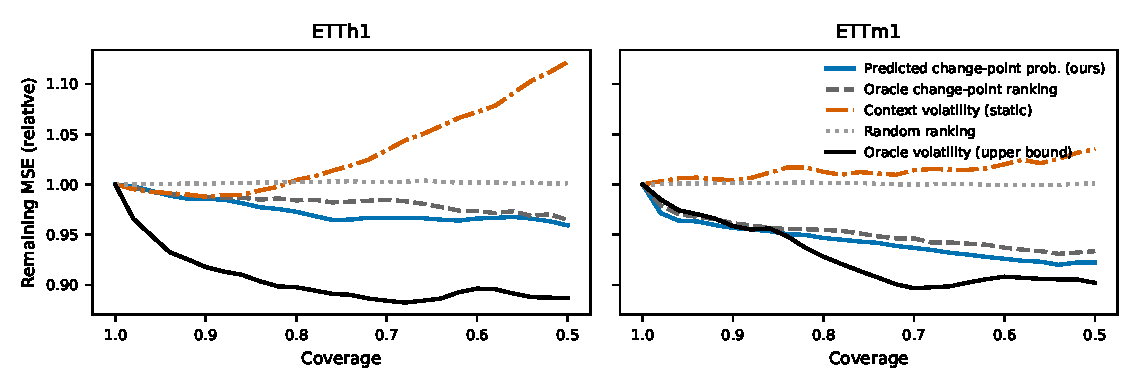
\includegraphics[width=0.55\linewidth]{figures/fig_riskcov.pdf}
  \caption{Risk--coverage curves on ETTh1, ETTm1, and fine-tuned Chronos-Bolt. Predicted change-point probability (blue) reduces remaining MSE monotonically, beating oracle change-point ranking (gray), context volatility (red), and random ranking (dashed); oracle volatility (black) marks the exploitable upper bound.}
  \label{fig:riskcov}
\end{figure}


\section{Discussion and Conclusion}
\label{sec:discussion}

\paragraph{Limitations.}
Positive repair evidence concentrates on positive-gap or lag-positive pairs, and several natural mechanisms for exploiting future-structure information do not work (Appendix~\ref{app:negative}): conditioning the forecast on predicted structure, per-window gating, scaling descriptor supervision to foundation-model fine-tuning, and supervising the future mean level. The descriptor's volatility channel is much weaker than its change-point channel. All experiments are point-forecasting; distributional extension is the natural next step.

Over-smoothing is not one phenomenon but two: rational shrinkage is the price of honest uncertainty; unexploited structure is repairable. The oracle gap tells them apart cheaply and predicts when anti-smoothing pays (14 of 15 cells, the exception diagnosable in advance): where it pays, a region-weighted loss recovers part of the structure; where not, a descriptor head reports when the forecast deserves trust.


\bibliographystyle{iclr2027_conference}
\bibliography{refs}

\section*{Reproducibility Statement}
All training protocols, backbone configurations, seeds, and compute details are documented in Appendix~\ref{app:repro}, and the diagnostic protocol in Appendix~\ref{app:diagnostic}. Code, experiment scripts, and the full 665-cell audit matrix are released in the accompanying repository.

\section*{Ethics Statement}
The study uses public benchmarks only and involves no human subjects or personal data. In high-stakes deployments of selective prediction, abstained windows should remain under human oversight or a validated fallback forecaster.

\appendix
\section{Proofs and Derivations}
\label{app:proofs}

\paragraph{Proof of Proposition~\ref{prop:oracle}.}
By orthogonality of the conditional mean, $\mathbb{E}\|y - m\|^2 = \mathbb{E}\|y - \mu + \mu - m\|^2 = \mathbb{E}\|\mu - m\|^2 + \mathbb{E}\,\mathrm{tr}\,\Sigma(x)$, since $\mathbb{E}[\langle \varepsilon, \mu - m \rangle] = 0$. The optimal forecast satisfies $\mathbb{E}\|\hat{y}^\star - m\|^2 = \mathbb{E}\|\mu - m\|^2$, which is strictly smaller whenever unpredictable variance exists. The amplitude-ratio bound follows from $\mathrm{Var}(y) = \mathrm{Var}(\mu) + \bar{\sigma}^2$ and $\mathrm{std}(\hat{y}^\star)^2 \le \mathrm{Var}(\mu)$.

\paragraph{Proof of Proposition~\ref{prop:interval}.}
Expand $\mathbb{E}\|\hat{y} + \delta - y\|^2 = \mathbb{E}\|\hat{y} - y\|^2 + 2\langle \delta, \mathbb{E}[\hat{y} - y] \rangle + |\delta|^2$. Since $\mathbb{E}[\hat{y} - y \mid x] = -b(x)$, the cross term equals $-2\langle \delta, b\rangle$, giving $\Delta\mathcal{L} = |\delta|^2 - 2\langle\delta, b\rangle$. The right side is negative exactly when $|\delta| < 2|b|\cos\theta$, and minimized at $\delta^\star = b$.

\paragraph{Derivation of the Gaussian fixed point \eqref{eq:fixedpoint}.}
With $w(y) = 1 + \alpha\mathbf{1}[y > c]$, the first-order condition $c = \mathbb{E}[w(y)\,y] / \mathbb{E}[w(y)]$ gives
\begin{equation}
    c = \frac{\mu + \alpha\left(\mu\,\bar{\Phi}(t) + \sigma\varphi(t)\right)}{1 + \alpha\,\bar{\Phi}(t)},
    \qquad t = \frac{c - \mu}{\sigma},
\end{equation}
using the truncated normal moments $\mathbb{E}[y \mid y > c] = \mu + \sigma\varphi(t)/\bar{\Phi}(t)$. At $t = 0$, the right-hand side exceeds $\mu$ by $\alpha\sigma\varphi(0)/(1 + \alpha/2)$, and a first-order expansion of the fixed point gives \eqref{eq:fixedpoint}. The $0.4\alpha\sigma$ form quoted in the main text is the small-$\alpha$ slope of this fixed point; the exact shift at $\alpha = 1$ is $0.27\sigma$, so the quoted form is an upper bound on the correction magnitude for $\alpha \le 1$. When the anchor equals $\mu$, the objective is symmetric about $\mu$ and develops minima at $\mu \pm \delta(\alpha)$, a double-well bifurcation that explains the anchor's role in controlling the correction's symmetry.

\section{Diagnostic Protocol Details}
\label{app:diagnostic}

\TBD{anchor sensitivity table (context mean versus seasonal naive), window-set sensitivity (tail versus sliding), bootstrap repetition convergence, and per-dataset gap table with confidence intervals.}

\section{Full Audit Matrix}
\label{app:matrix}

\begin{table}[h]
  \small
  \caption{Backbone-level law check on Electricity (PatchTST-family region-weighted repair, $\alpha{=}1$). The per-backbone oracle gap, not the architecture family, orders the outcomes.}
  \label{tab:backbone}
  \centering
  \begin{tabular}{lccc}
    \toprule
    Backbone & Oracle gap & $\Delta$MSE (\%) & Consistent \\
    \midrule
    PatchTST & $+0.030$ & $-2.3$ & \checkmark \\
    DLinear & $+0.005$ & $+1.9$ & \checkmark \\
    TimeMixer & $-0.008$ & $+1.7$ & \checkmark \\
    TimesNet & $-0.034$ & $+4.3$ & \checkmark \\
    iTransformer & $-0.031$ & $+4.3$ & \checkmark \\
    \bottomrule
  \end{tabular}
\end{table}

\TBD{the complete 665-cell oracle-gap matrix, generated from \texttt{gapbench/results/matrix.csv}.}

\section{Implementation and Reproducibility}
\label{app:repro}

\TBD{backbone configurations, training protocol, optimizer settings, descriptor-head specification, region-loss hyperparameters, and compute summary.}


\end{document}
